\documentclass{article}
\usepackage[a4paper, portrait, margin=1.1811in]{geometry}
\usepackage[english]{babel}
\usepackage[utf8]{inputenc}
\usepackage[T1]{fontenc}
\usepackage{helvet}
\usepackage{etoolbox}
\usepackage{graphicx}
\usepackage{titlesec}
\usepackage{caption}
\usepackage{booktabs}
\usepackage{xcolor} 
\usepackage{adjustbox}
\usepackage[colorlinks, citecolor=cyan]{hyperref}
\usepackage{caption}
\captionsetup[figure]{name=Figure}
\graphicspath{ {./images/} }
\usepackage{scrextend}
\usepackage{fancyhdr}
\usepackage{graphicx}
\newcounter{lemma}
\newtheorem{lemma}{Lemma}
\newcounter{theorem}
\newtheorem{theorem}{Theorem}

\fancypagestyle{plain}{
	\fancyhf{}
	\renewcommand{\headrulewidth}{0pt}
	\renewcommand{\familydefault}{\sfdefault}
}

%\pagestyle{plain}
\makeatletter
\patchcmd{\@maketitle}{\LARGE \@title}{\fontsize{16}{19.2}\selectfont\@title}{}{}
\makeatother

\usepackage{authblk}
\renewcommand\Authfont{\fontsize{10}{10.8}\selectfont}
\renewcommand\Affilfont{\fontsize{10}{10.8}\selectfont}
\renewcommand*{\Authsep}{, }
\renewcommand*{\Authand}{, }
\renewcommand*{\Authands}{, }
\setlength{\affilsep}{2em}  
\newsavebox\affbox
\author{\textbf{Olteanu Fabian Cristian}}
\affil{FMI, AI Master, Year 2
}

\titlespacing\section{0pt}{12pt plus 4pt minus 2pt}{0pt plus 2pt minus 2pt}
\titlespacing\subsection{12pt}{12pt plus 4pt minus 2pt}{0pt plus 2pt minus 2pt}
\titlespacing\subsubsection{12pt}{12pt plus 4pt minus 2pt}{0pt plus 2pt minus 2pt}


\titleformat{\section}{\normalfont\fontsize{10}{15}\bfseries}{\thesection.}{1em}{}
\titleformat{\subsection}{\normalfont\fontsize{10}{15}\bfseries}{\thesubsection.}{1em}{}
\titleformat{\subsubsection}{\normalfont\fontsize{10}{15}\bfseries}{\thesubsubsection.}{1em}{}

\titleformat{\author}{\normalfont\fontsize{10}{15}\bfseries}{\thesection}{1em}{}

\title{\textbf{\huge Deep Learning Project 2 Report}}
\date{}    

\begin{document}

\pagestyle{headings}	
\newpage
\setcounter{page}{1}
\renewcommand{\thepage}{\arabic{page}}


	
\captionsetup[figure]{labelfont={bf},labelformat={default},labelsep=period,name={Figure }}	\captionsetup[table]{labelfont={bf},labelformat={default},labelsep=period,name={Table }}
\setlength{\parskip}{0.5em}
	
\maketitle
	
\noindent\rule{15cm}{0.4pt}

\section{Introduction}
The task at hand is to classify a set of images containing 150 different Pokemon. The dataset contains roughly 7000 samples. The methods that were used to perform this task were three different convolutional network architectures.

\section{Dataset}
The dataset is imbalanced, as shown in the histogram below (fig 1). As such, data augmentation was used to compensate this fact. For the training data generator, various augmentation techniques such as rotation, zooming, shifting, shearing, and flipping are applied to increase the diversity of training samples and improve the model's generalization. The testing data generator only applies rescaling to normalize pixel values.

\begin{figure}[hbt!]
	\centering
	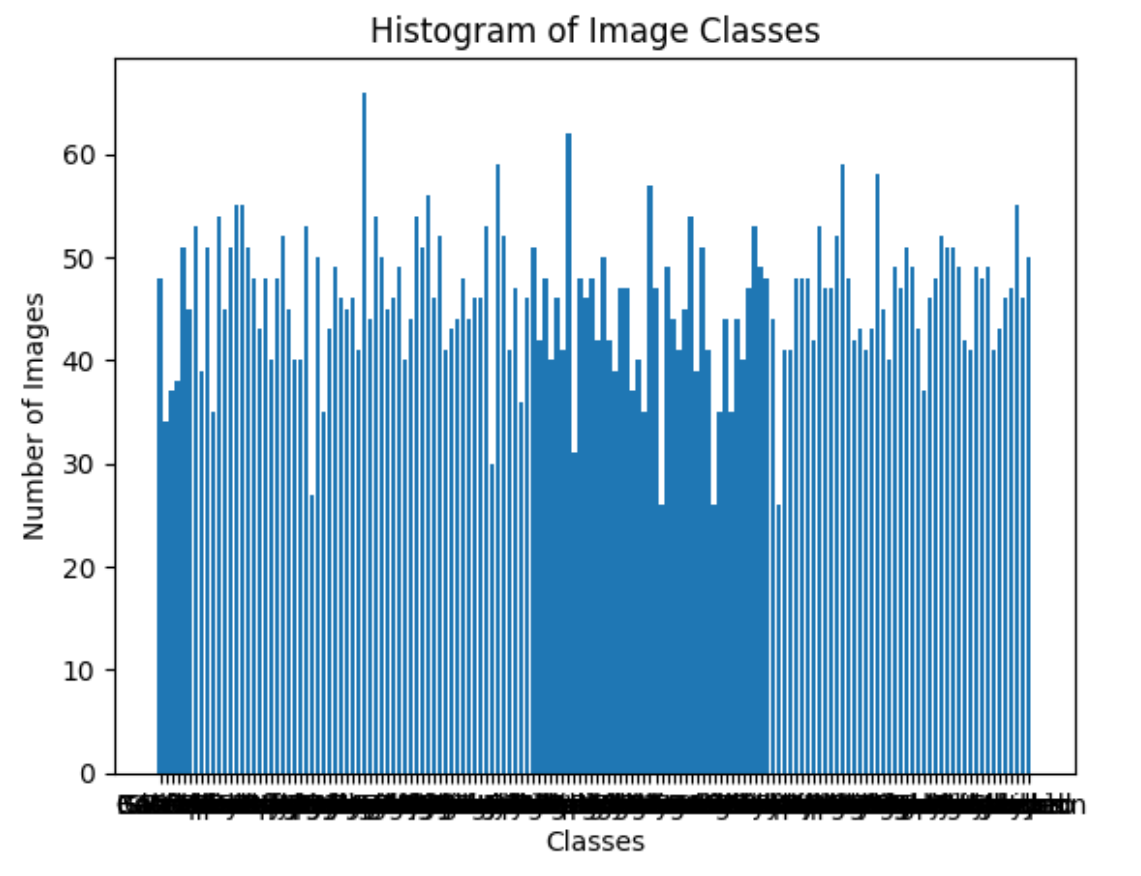
\includegraphics[scale=0.30]{dataset_histogram.png}
	\caption{Dataset histogram}
\end{figure}

Before training any models using this dataset, it was split into three folds: train, validation and test using the following ratios: 0.75, 0.15 and 0.1.

\section{VGG16 Implementation}
VGG16 is a classic CNN architecture known for its simplicity and effectiveness. It consists of 13 convolutional layers and 3 fully connected layers. The architecture is characterized by stacking multiple 3x3 convolutional layers followed by max-pooling layers. Batch normalization is applied after each convolutional layer to stabilize and accelerate the training process. The VGG16 architecture is trained on the Pokemon dataset using stochastic gradient descent (SGD) optimizer with a learning rate of 0.001. The model is compiled with categorical cross-entropy loss and evaluated based on accuracy and F1-score metrics. In the case of training it from scratch on this dataset, however, it yielded very poor results (and so did AlexNet).

\subsection{Comparison with the original paper}
Comparing this architecture to the original\cite{vgg16}, the most obvious change becomes apparent when looking at the added batch normalization layers, which were added after some initial tries when the model wouldn't learn. Additionally, the input layer was adapted to 64 by 64, which is different from the original VGG16 input layer, which accepted 224 by 224 images.

\section{AlexNet Implemention}
AlexNet\cite{alexnet} is a pioneering CNN architecture that significantly contributed to the advancement of deep learning in computer vision. It consists of eight layers, including five convolutional layers and three fully connected layers. The architecture incorporates overlapping max-pooling and dropout regularization to prevent overfitting. The AlexNet model for Pokemon classification is trained using SGD optimizer with a learning rate of 0.001. It is compiled with categorical cross-entropy loss and evaluated based on accuracy and F1-score.

Below, the original architecture is described, along with comparisons to the actual implementation in this project:

\begin{itemize}
\item AlexNet takes input images of size 227x227x3 (227 pixels in height and width, with three color channels for Red, Green, and Blue). In the implementation, this was changed to 64x64x3, as this was the size of the preprocessed images.
\item AlexNet consists of five convolutional layers, denoted as Conv1 to Conv5. These layers extract features from the input images using learned filters.
\item Conv1: 96 filters of size 11x11x3 with a stride of 4
\item Conv2: 256 filters of size 5x5x48 (48 channels are the output from the first layer) with a stride of 1.
\item Conv3: 384 filters of size 3x3x256 with a stride of 1.
\item Conv4: 384 filters of size 3x3x192 with a stride of 1.
\item Conv5: 256 filters of size 3x3x192 with a stride of 1.
\item Note: The custom AlexNet implementation uses different filter sizes and strides for max-pooling compared to the original AlexNet. Additionally, the implementation in this project includes batch normalization layers after each convolutional layer, which one would have believed that it would help in stabilizing and accelerating the training process.
\item ReLU (Rectified Linear Unit) activation functions are applied after each convolutional layer to introduce non-linearity.
\item There are three max-pooling layers in AlexNet. These layers downsample the feature maps obtained from the convolutional layers to reduce spatial dimensions. Each has a filter size of 3x3 and a stride of 2.
\item After the convolutional and max-pooling layers, there are three fully connected layers. The first two contain 4096 neurons and the last one contains a number of units equal to the number of classes (1000 in the original paper, as it was used on the ImageNet dataset), which, in our case, is 150.
\item Dropout regularization is not explicitly included in the implementation in this project, whereas AlexNet applies dropout to the fully connected layers.
\item The output layer employs the softmax activation function to generate class probabilities for the input image.
\end{itemize}
\section{Custom CNN Implementation}
The last model that was tried was a custom convolutional neural network, which follows this architecture:
\begin{itemize}
\item Four convolutional blocks are used with the following configuration: 
\begin{enumerate}
\item a 2-D convolution layer is applied with 64 filters, 3 by 3 kernel size and same padding and uses the ReLU activation function
\item a batch normalization layer is then applied
\item max pooling 2D is then applied, with a 2 by 2 pool size
\end{enumerate}
\item A fully connected layer of 512 neurons is applied to the flattened output of the last convolutional layer.

\item An output layer with softmax activation is then applied to obtain the label predictions.
\end{itemize}
The model is compiled using the adam optimizer and categorical crossentropy as its loss function and uses the F1 score in addition to accuracy as training-time evaluation metrics.

\section{Results}
Surprisingly, the AlexNet and VGG16 implementations performed extremely poorly, with accuracies of 0.0398 and, respectively, 0.0099 on the test set. The custom cnn implementation, however, did much better as its accuracy was 0.5789 on the test set. Figures 2, 3 and 4 depict the confusion matrices for the three models on the test set.

\begin{figure}[hbt!]
	\centering
	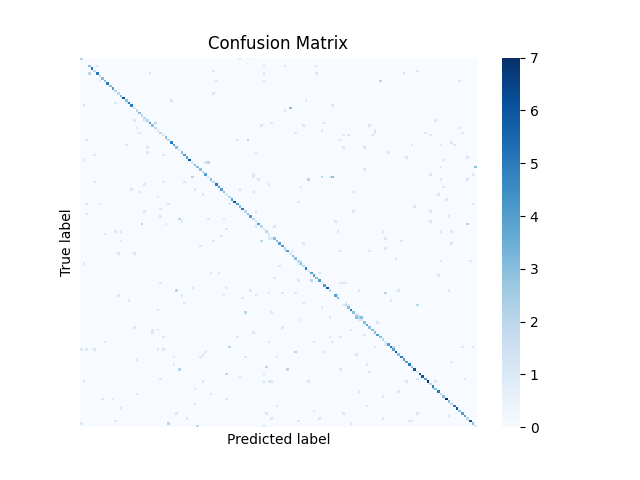
\includegraphics[scale=0.58]{../conf_matrices/cnn_conf_matrix.png}
	\caption{Custom CNN Confusion Matrix on the Test Set}
\end{figure}

\begin{figure}[hbt!]
	\centering
	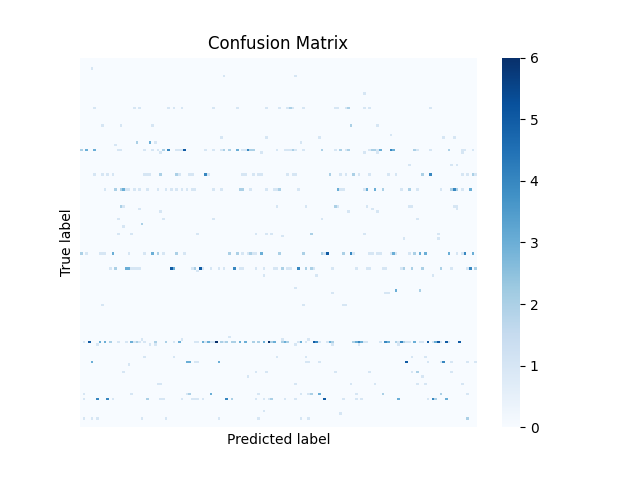
\includegraphics[scale=0.58]{../conf_matrices/vgg16_conf_matrix.png}
	\caption{VGG16 Matrix on the Test Set}
\end{figure}

\begin{figure}[hbt!]
	\centering
	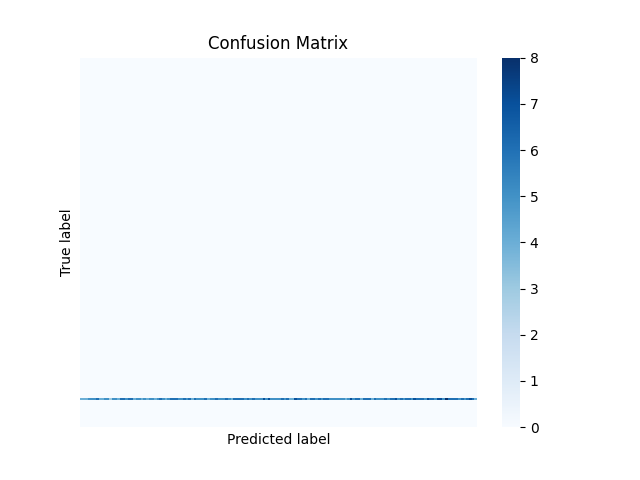
\includegraphics[scale=0.58]{../conf_matrices/alexnet_conf_matrix.png}
	\caption{AlexNet Matrix on the Test Set}
\end{figure}

\newpage 

\section{Conclusion}
The technical analysis of the Custom CNN, VGG16 and AlexNet models reveals the fact that the former two were very unfit for this task, as the custom network gave much better predictions as opposed to the others.

\newpage

\bibliographystyle{IEEEtran}

%\bibliography{template} %-->reference list is on the template.bib file
\begin{thebibliography}{1.7} 
	\bibitem{vgg16}Simonyan, K. \& Zisserman, A. Very Deep Convolutional Networks for Large-Scale Image Recognition.  (2015)
	\bibitem{alexnet}Krizhevsky, A., Sutskever, I. \& Hinton, G. ImageNet classification with deep convolutional neural networks. {\em Proceedings Of The 25th International Conference On Neural Information Processing Systems - Volume 1}. pp. 1097-1105 (2012)


\end{thebibliography}

\end{document}